%! Author = wolfram_e_laube
%! Date = 06.05.24

\item[(c)]
\section{Exercise 1 Task (c): Visualization of Continuous and Sampled Signals}

\subsection{Problem Statement}
This task involves plotting the analog signal $x(t)$, emulated at a high sampling rate to approximate continuous behavior, and the corresponding sampled signal $x[n]$ over a 2 ms interval. The goal is to visually demonstrate that $x[n]$ accurately represents $x(t)$, confirming the effects seen in the spectral analysis from Task (b).

\subsection{Signal Definition}
The signal $x(t)$ is defined as:
$$
x(t) = \sin(2\pi 4000 t) + \sin(2\pi 6000 t),
$$
where $f_1 = 4000 \text{ Hz}$ and $f_2 = 6000 \text{ Hz}$. It is sampled at a rate of 10 kHz to produce $x[n]$.

\subsection{Conclusion}
The resulting plot demonstrates that the sampled signal $x[n]$ at 10 kHz captures the waveform of the continuous signal $x(t)$ effectively. The discrete points align well with the peaks and troughs of the emulated analog signal, confirming the sufficiency of the sampling rate and corroborating the spectral analysis presented in Task (b).

\begin{figure}[h]
    \centering
    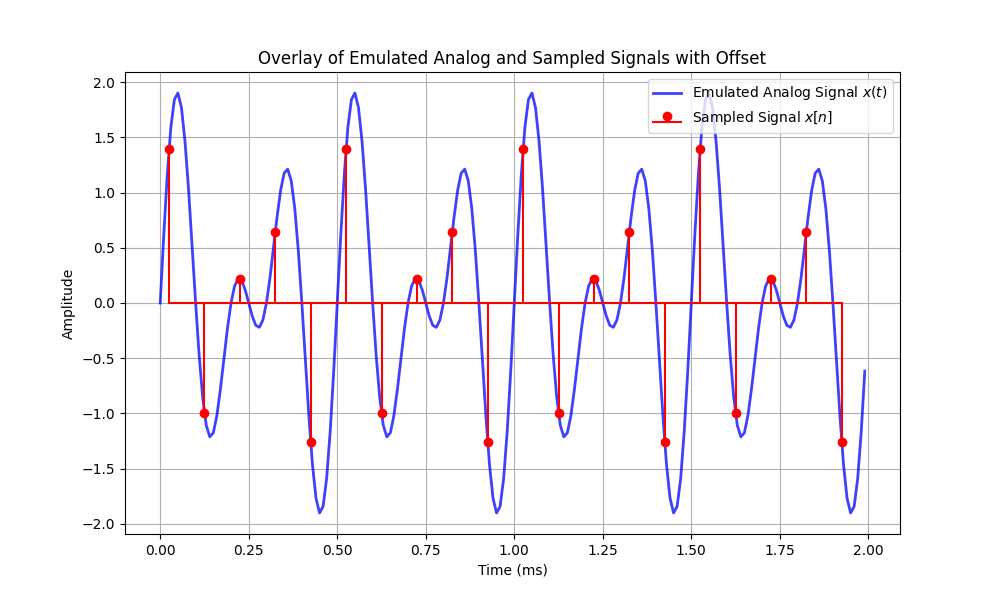
\includegraphics[width=0.49\textwidth]{fig/ex1_c_plot_1}
    \caption{Analog and Sampled Signals of \(x(t)\)}
    \label{fig:ex1_c_plot_1}
\end{figure}

\begin{figure}[h]
    \centering
    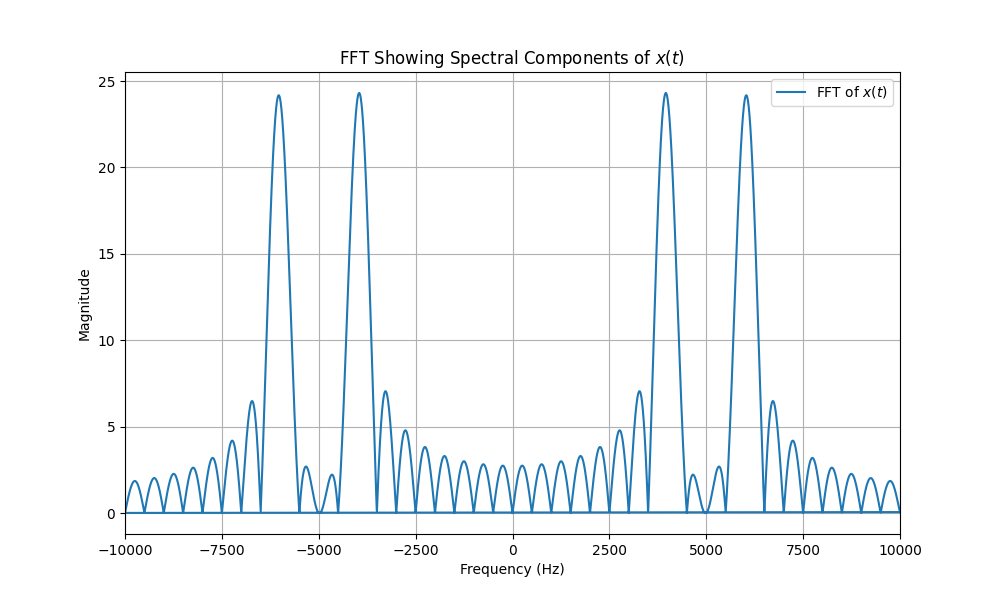
\includegraphics[width=0.49\textwidth]{fig/ex1_c_plot_2}
    \caption{Analog and Sampled Signals of \(x(t)\)}
    \label{fig:ex1_c_plot_2}
\end{figure}
